\documentclass{article}
\usepackage{tikz}
\usepackage{amsmath, empheq}
\begin{document}
    % TikZ picture with origin upper left
    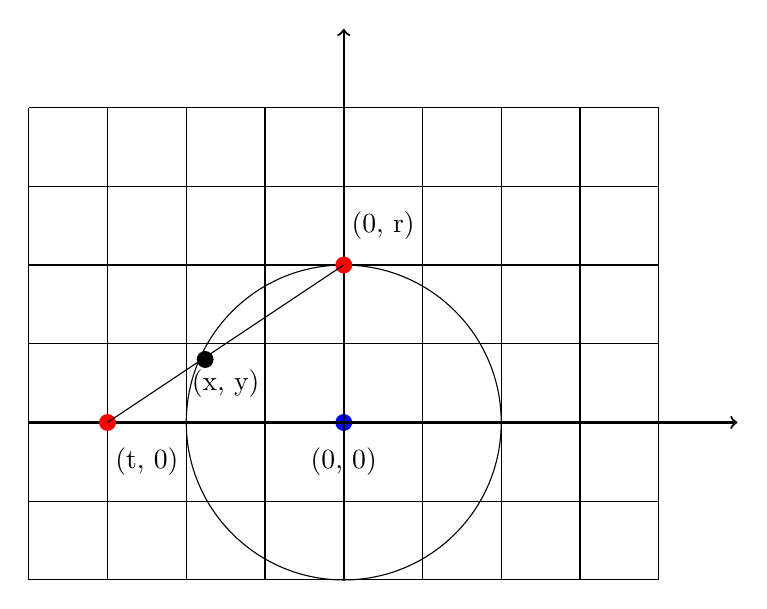
\begin{tikzpicture}[yscale=-1] 
        % 4x4 grid
        \draw (-2, 0) grid (6, 6);
        % origin point
        \draw [color=blue, fill=blue] (2, 4) circle (0.1);
        % x-axis
        \draw [thick,->] (-2, 4) -- (7, 4);
        % y-axis
        \draw [thick,->] (2, 6) -- (2, -1);
        % origin label
        \node at (2, 4.5) {(0, 0)};
        \draw (2, 4) circle (2);
        \draw [color=red, fill=red] (2, 2) circle(0.1);
        \node at (2.5, 1.5){(0, r)};
        \draw [color=red, fill=red] (-1, 4) circle(0.1);
        \node at (-0.5, 4.5){(t, 0)};
        \draw (2, 2)--(-1, 4);
        \node at (0.5, 3.5){(x, y)};
        \draw [color=black, fill=black] (0.24, 3.2) circle(0.1);
    \end{tikzpicture}\\ \\
	\centerline{Derive circle parametric equation}
	\begin{flalign*}
	\textit{Line equation from (0,r) to (t, 0)}\quad
	\frac{y-0}{x-t}=\frac{y-r}{x-0}\\
    \Rightarrow xy=(y - r)(x - t)  \\
   \Rightarrow xy=xy - rx - yt + rt\\
	\Rightarrow  rx=rt-yt=t(r-y) \\
	\Rightarrow  rx = t(r-y)\\
	\Rightarrow x = \frac{t}{r}(r-y) \tag{1}\\
	\textit{Let the circle equation to be}\\
	 x^{2} + y^{2} = r^{2} \tag{2}\\
	\Rightarrow \left (\frac{t}{r}(r-y)  \right )^{2} + y^{2}=r^{2}\\
	\Rightarrow \left (\frac{t}{r} \right )^{2}(r-y)^{2} + y^{2}=r^{2}\\
	\Rightarrow t^{2}(r^{2}+y^{2}-2ry) + r^{2}y^{2} = r^{4}\\
	\Rightarrow t^{2}r^{2} + t^{2}y^{2} - 2rt^{2}y + r^{2}y^{2}=r^{4}\\
	\Rightarrow (t^{2}+r^{2})y^{2} - 2rt^{2}y + t^{2}r^{2}-r^{4}=0\\
	 \end{flalign*}
	 \begin{flalign*}
	\Rightarrow a=(t^{2}+r^{2})\quad b=-2rt^{2}\quad c=t^{2}r^{2}-r^{4}\\
	y=\frac{-b\pm\sqrt{b^{2}-4ac}}{2a}\\
	\Rightarrow y=\frac{2rt^{2}\pm\sqrt{4r^{2}t^{4}-4(t^{2}+r^{2})(t^{2}r^{2}-r^{4})}}{2(t^{2}+r^{2})}\\
	\Rightarrow y=\frac{rt^{2}\pm \sqrt{r^{2}t^{4}-( t^{4}r^{2} - t^{2}r^{4} + t^{2}r^{4} - r^{6} )}}{(t^{2}+r^{2})}\\
	\Rightarrow y=\frac{rt^{2}\pm \sqrt{r^{2}t^{4} - t^{4}r^{2} + t^{2}r^{4} - t^{2}r^{4} + r^{6} }}{(t^{2}+r^{2})}\\
	\Rightarrow y=\frac{rt^{2}\pm \sqrt{ t^{2}r^{4} - t^{2}r^{4} + r^{6} }}{(t^{2}+r^{2})}\\
	\Rightarrow y=\frac{r(t^{2}\pm r^{2})}{(t^{2}+r^{2})}\\
		y=r \text{ or } y=\frac{r(t^{2} - r^{2})}{(t^{2}+r^{2})}\\
\text{If }\quad y=r\quad\Rightarrow
\begin{minipage}{0.45\textwidth}
	\begin{empheq}[left=\empheqlbrace]{align*}
		x = \frac{t}{r}(r-y) = 0\\
		y=r
	\end{empheq}
\end{minipage}\\
\text{If }\quad  y=\frac{r(t^{2} - r^{2})}{(t^{2}+r^{2})} \quad\Rightarrow
\begin{minipage}{0.45\textwidth}
	\begin{empheq}[left=\empheqlbrace]{align*}
		x = \frac{t}{r}(r-y) \tag{2}\\
		y=\frac{r(t^{2} - r^{2})}{(t^{2}+r^{2})} \tag{3}
	\end{empheq}
\end{minipage}\\
\text{ Sub(3) into (2)}\\
\Rightarrow x=\frac{t}{r}\left (r- \frac{r(t^{2}-r^{2})}{t^{2}+r^{2}}  \right) \\
\Rightarrow x= t \left(1-\frac{(t^{2}-r^{2})}{t^{2}+r^{2}} \right)\\
\Rightarrow x= \frac{2tr^{2}}{t^{2}+r^{2}}\\
\Rightarrow
\begin{minipage}{0.45\textwidth}
	\begin{empheq}[left=\empheqlbrace]{align*}
		x= r\frac{2tr}{t^{2}+r^{2}} \\
		y= r\frac{(t^{2} - r^{2})}{t^{2}+r^{2}}
	\end{empheq}
\end{minipage}
{ or }
\begin{minipage}{0.45\textwidth}
	\begin{empheq}[left=\empheqlbrace]{align*}
		x= 0 \\
		y= r
	\end{empheq}
\end{minipage}
\end{flalign*}
\end{document}
